\documentclass[12pt]{article}
\usepackage[margin=1in]{geometry}
\usepackage{cite}
\usepackage{amsmath,amssymb,amsfonts}
\usepackage{graphicx}
\usepackage{booktabs}
\usepackage{hyperref}
\usepackage{setspace}
\usepackage{caption}
\usepackage{subcaption}
\usepackage{float}
\usepackage{xcolor}
\usepackage{array}
\usepackage{colortbl}
\usepackage{microtype}

\onehalfspacing

\definecolor{wingreen}{rgb}{0.13, 0.55, 0.13}
\definecolor{lightgray}{gray}{0.93}
\definecolor{colA}{RGB}{44,123,182}
\definecolor{colB}{RGB}{26,150,65}
\definecolor{colC}{RGB}{244,109,67}
\definecolor{colD}{RGB}{123,45,139}

\hypersetup{colorlinks=true, linkcolor=black, citecolor=black, urlcolor=blue}

\title{\textbf{\Large Scale vs.\ Architecture: A 2$\times$2 Empirical Study of\\
Model Size and Pipeline Design in Retrieval-Augmented Generation}}
\author{Ahmad Tawil \\ \texttt{ahmadtawil.se@gmail.com}}
\date{May 2026}

\begin{document}
\maketitle

%──────────────────────────────────────────────────────────────────────────────
\begin{abstract}
%──────────────────────────────────────────────────────────────────────────────
The prevailing assumption in Retrieval-Augmented Generation (RAG) is that
larger models and more sophisticated pipelines always produce better results.
This paper challenges that assumption with a controlled 2$\times$2 factorial
experiment on the HotpotQA multi-hop question-answering benchmark, crossing
two model families (GPT-5.4-mini and Llama-3.1-8B) with two pipeline
architectures (naive single-pass RAG and agentic self-correcting RAG).
The four systems---Goliath (Naive~GPT), David (Agentic~Llama), Hermes
(Naive~Llama), and Titan (Agentic~GPT)---are evaluated on 100 questions
across exact-match accuracy and four RAGAS metrics.

The headline finding is a substantial \textbf{model-by-pipeline interaction
effect}: agentic self-correction \emph{helps} GPT-5.4-mini ($+6.0$ percentage
points in exact-match) but \emph{hurts} Llama-3.1-8B ($-7.0$pp), revealing
that iterative self-correction imposes a reasoning demand that smaller models
cannot reliably satisfy.  Surprisingly, Hermes (Naive Llama) achieves the
highest overall exact-match accuracy of all four systems (65.0\%), outperforming
all GPT variants on this metric.  On RAGAS metrics, Titan (Agentic GPT) leads
in answer relevancy, context precision, and context recall, while Hermes leads
in faithfulness.  All four systems achieved 100\% completion rate, enabled by
running inference on a local GPU (NVIDIA Tesla T4) via Ollama, eliminating the
rate-limit failures that plagued earlier work.

These results suggest that for smaller models, architectural complexity is a
liability rather than an asset, and that the decision to deploy an agentic
pipeline should be conditioned on the underlying model's self-correction
capability.
\end{abstract}

\noindent\textbf{Keywords:} Retrieval-Augmented Generation, Agentic AI,
Self-Correction, Multi-Hop Question Answering, HotpotQA, LangGraph,
LLM Evaluation, RAGAS, Model Scale, Pipeline Architecture

%──────────────────────────────────────────────────────────────────────────────
\section{Introduction}
%──────────────────────────────────────────────────────────────────────────────

The scaling hypothesis---that more parameters yield better outputs---has
dominated NLP research for the past decade~\cite{brown2020gpt3,kaplan2020scaling}.
In the RAG setting, this translates to the common engineering practice of
coupling the largest affordable frontier model with a simple retrieve-then-generate
pipeline.  A parallel line of work has shown that \emph{how} a model reasons
may matter as much as \emph{how large} it is: agentic systems that iterate,
self-check, and reformulate their queries achieve strong results on multi-step
reasoning tasks~\cite{yao2022react,shinn2023reflexion,asai2023selfrag}.

Prior work typically evaluates scale and architecture in isolation.  In this
paper I ask a more precise question: \emph{do scale and pipeline architecture
interact?}  Specifically, does an agentic pipeline provide the same benefit
regardless of the underlying model's capability, or does it require a certain
level of reasoning competence to function correctly?

I answer this empirically with a \textbf{2$\times$2 factorial design}:

\begin{center}
\begin{tabular}{lcc}
\toprule
 & \textbf{Naive Pipeline} & \textbf{Agentic Pipeline} \\
\midrule
\textbf{GPT-5.4-mini} & System A (Goliath) & System D (Titan) \\
\textbf{Llama-3.1-8B} & System C (Hermes)  & System B (David)  \\
\bottomrule
\end{tabular}
\end{center}

All four systems share identical embeddings, vector store, retrieval
configuration, and benchmark, isolating model choice and pipeline architecture
as the sole independent variables.

My \textbf{contributions} are:
\begin{enumerate}
    \item I conduct the first controlled 2$\times$2 factorial comparison of
          model scale and pipeline architecture in RAG, on the HotpotQA
          distractor benchmark.
    \item I observe an \textbf{interaction effect}: agentic
          self-correction benefits capable models but harms smaller ones,
          suggesting a \emph{capability threshold} for productive self-correction.
    \item I show that Naive Llama achieves the highest exact-match accuracy
          of all four systems, challenging the assumption that architectural
          sophistication always helps.
    \item I demonstrate 100\% completion across all systems by eliminating
          API rate limits through local GPU inference (NVIDIA Tesla T4 via
          Ollama), removing a confound present in earlier studies.
\end{enumerate}

%──────────────────────────────────────────────────────────────────────────────
\section{Related Work}
%──────────────────────────────────────────────────────────────────────────────

\subsection{Retrieval-Augmented Generation}
Lewis et al.~\cite{lewis2020retrieval} introduced the canonical RAG architecture,
demonstrating that augmenting generation with retrieved passages substantially
reduces hallucination on knowledge-intensive tasks.  Subsequent work improved
retrieval quality via dense passage retrieval~\cite{karpukhin2020dense} and
hybrid sparse-dense strategies.  Most practical deployments still follow the
original single-pass retrieve-then-generate paradigm (our ``naive'' baseline).

\subsection{Agentic and Iterative Reasoning}
ReAct~\cite{yao2022react} showed that interleaving reasoning traces with
action execution improves multi-step task performance.  Reflexion~\cite{shinn2023reflexion}
extended this with verbal self-reflection.  Self-RAG~\cite{asai2023selfrag}
introduced critic tokens that allow a model to decide when to retrieve,
evaluate retrieved passages, and verify its own output---a conceptual precursor
to the agentic pipeline implemented in this work.  Critically, these prior
works do not systematically study whether the benefit of agentic iteration
depends on the capability of the underlying model.

\subsection{Multi-Hop Question Answering}
HotpotQA~\cite{yang2018hotpotqa} requires reasoning over two or more Wikipedia
paragraphs.  The distractor setting presents 10 paragraphs per question
(2 gold, 8 irrelevant), specifically to test whether a system can identify
relevant evidence rather than treating all retrieved text as equally useful.
This makes HotpotQA especially sensitive to the document-grading component of
agentic pipelines.

\subsection{RAG Evaluation}
Traditional n-gram metrics (BLEU, ROUGE) do not capture factual grounding
quality.  The RAGAS framework~\cite{es2023ragas} addresses this with four
LLM-as-judge metrics: \emph{faithfulness}, \emph{answer relevancy},
\emph{context precision}, and \emph{context recall}.

%──────────────────────────────────────────────────────────────────────────────
\section{Methodology}
%──────────────────────────────────────────────────────────────────────────────

\subsection{System Architectures}

\subsubsection{System A --- Goliath: Naive RAG with GPT-5.4-mini}

The standard single-pass pipeline: embed question $\rightarrow$ retrieve top-5
passages from ChromaDB $\rightarrow$ generate answer with GPT-5.4-mini.  No
document grading, query reformulation, or post-generation verification.  This
represents the most common RAG implementation found in production today.

\subsubsection{System B --- David: Agentic RAG with Llama-3.1-8B}

A cyclic directed graph implemented with LangGraph.  The same model
(Llama-3.1-8B served via Ollama on a Tesla T4 GPU) performs all agentic
reasoning steps: document grading, query rewriting, generation, and
hallucination verification.  The pipeline state tracks retrieval and generation
attempt counts to enforce loop bounds.

\textbf{Control flow:} After grading, if documents are relevant $\rightarrow$
generate; else if retrieval attempts $< 3$ $\rightarrow$ rewrite query and
retry; else $\rightarrow$ generate from best available documents.  After
hallucination check, if answer is grounded $\rightarrow$ end; else if
generation attempts $< 2$ $\rightarrow$ regenerate; else $\rightarrow$ end.

\subsubsection{System C --- Hermes: Naive RAG with Llama-3.1-8B}

Identical single-pass pipeline as System A but using Llama-3.1-8B (via Ollama)
instead of GPT-5.4-mini.  This cell isolates the effect of model choice under
the naive pipeline.

\subsubsection{System D --- Titan: Agentic RAG with GPT-5.4-mini}

Identical agentic graph as System B but using GPT-5.4-mini (via OpenAI API)
for all reasoning steps.  This cell isolates the effect of pipeline architecture
with the more capable model.

\subsection{Shared Infrastructure}

All four systems share identical infrastructure to ensure a fair comparison:

\begin{itemize}
    \item \textbf{Embedding model:} \texttt{sentence-transformers/all-MiniLM-L6-v2},
          running locally on CPU with L2-normalised embeddings.
    \item \textbf{Vector store:} ChromaDB (\texttt{hotpotqa\_dev} collection),
          with per-question corpus scoping via \texttt{question\_id} metadata.
    \item \textbf{Retrieval:} Top-$k=5$ passages per query, filtered to the
          current question's 10-paragraph partition.
    \item \textbf{Chunking:} Paragraphs stored as single chunks
          (RecursiveCharacterTextSplitter, max 1{,}000 chars, 200-char overlap).
    \item \textbf{Temperature:} 0.0 for all LLM calls (deterministic).
\end{itemize}

\subsection{Inference Infrastructure}

Llama systems (B and C) run on a \textbf{NVIDIA Tesla T4 GPU} (15\,GiB VRAM)
via Ollama on Google Colab, using the \texttt{llama3.1:8b} quantised model
($\approx$5.4\,GiB VRAM).  GPT systems (A and D) call the OpenAI API.
This setup achieved 100\% completion for all four systems, resolving the
rate-limit failures reported in earlier work with cloud inference APIs.

\subsection{Dataset}

\begin{table}[H]
\centering
\caption{HotpotQA Benchmark Configuration}
\label{tab:dataset}
\begin{tabular}{ll}
\toprule
\textbf{Parameter} & \textbf{Value} \\
\midrule
Split              & Validation (distractor setting) \\
Sample size        & 100 questions \\
Random seed        & 42 \\
Difficulty         & Hard (all sampled questions) \\
Question types     & Bridge: 86 (86\%), Comparison: 14 (14\%) \\
Paragraphs ingested & 1{,}000 (100 $\times$ 10) \\
\bottomrule
\end{tabular}
\end{table}

\subsection{Evaluation Metrics}

\textbf{(1) Exact-Match Accuracy (EM):} The ground-truth answer string must
appear as a substring of the system's response.  A conservative metric that
provides a direct, reproducible comparison signal.

\textbf{(2) RAGAS Metrics:} Evaluated with GPT-5.4 as the judge LLM.  Four
metrics are computed for each system: \emph{faithfulness},
\emph{answer relevancy}, \emph{context precision}, and \emph{context recall},
each scored in $[0,1]$.  All four metrics computed successfully for all systems,
likely due to the updated RAGAS~0.4.x API and the slightly different 100-question
sample relative to earlier work.

%──────────────────────────────────────────────────────────────────────────────
\section{Results}
%──────────────────────────────────────────────────────────────────────────────

\subsection{Completion Rate}

All four systems completed all 100 questions (100\% completion rate).  This
is a significant improvement over earlier work, where Groq API rate limits
caused a 30.5\% failure rate for the agentic Llama system.  Running Llama
locally on a Tesla T4 GPU via Ollama eliminates this constraint entirely.

\subsection{Exact-Match Accuracy}

\begin{table}[H]
\centering
\caption{Exact-Match Accuracy by System and Question Type}
\label{tab:em}
\rowcolors{2}{lightgray}{white}
\begin{tabular}{lcccc}
\toprule
\textbf{System} & \textbf{Model} & \textbf{Pipeline} &
\textbf{Overall EM} & \textbf{Bridge / Comparison} \\
\midrule
A --- Goliath & GPT-5.4-mini & Naive   & 52.0\% & 50.0\% / 64.3\% \\
B --- David   & Llama-3.1-8B & Agentic & 58.0\% & 55.8\% / 71.4\% \\
\textcolor{wingreen}{\textbf{C --- Hermes}} &
  \textcolor{wingreen}{\textbf{Llama-3.1-8B}} &
  \textcolor{wingreen}{\textbf{Naive}}   &
  \textcolor{wingreen}{\textbf{65.0\%}} &
  \textcolor{wingreen}{\textbf{64.0\%}} / \textcolor{wingreen}{\textbf{71.4\%}} \\
D --- Titan   & GPT-5.4-mini & Agentic & 58.0\% & 55.8\% / 71.4\% \\
\bottomrule
\end{tabular}
\end{table}

\begin{figure}[H]
\centering
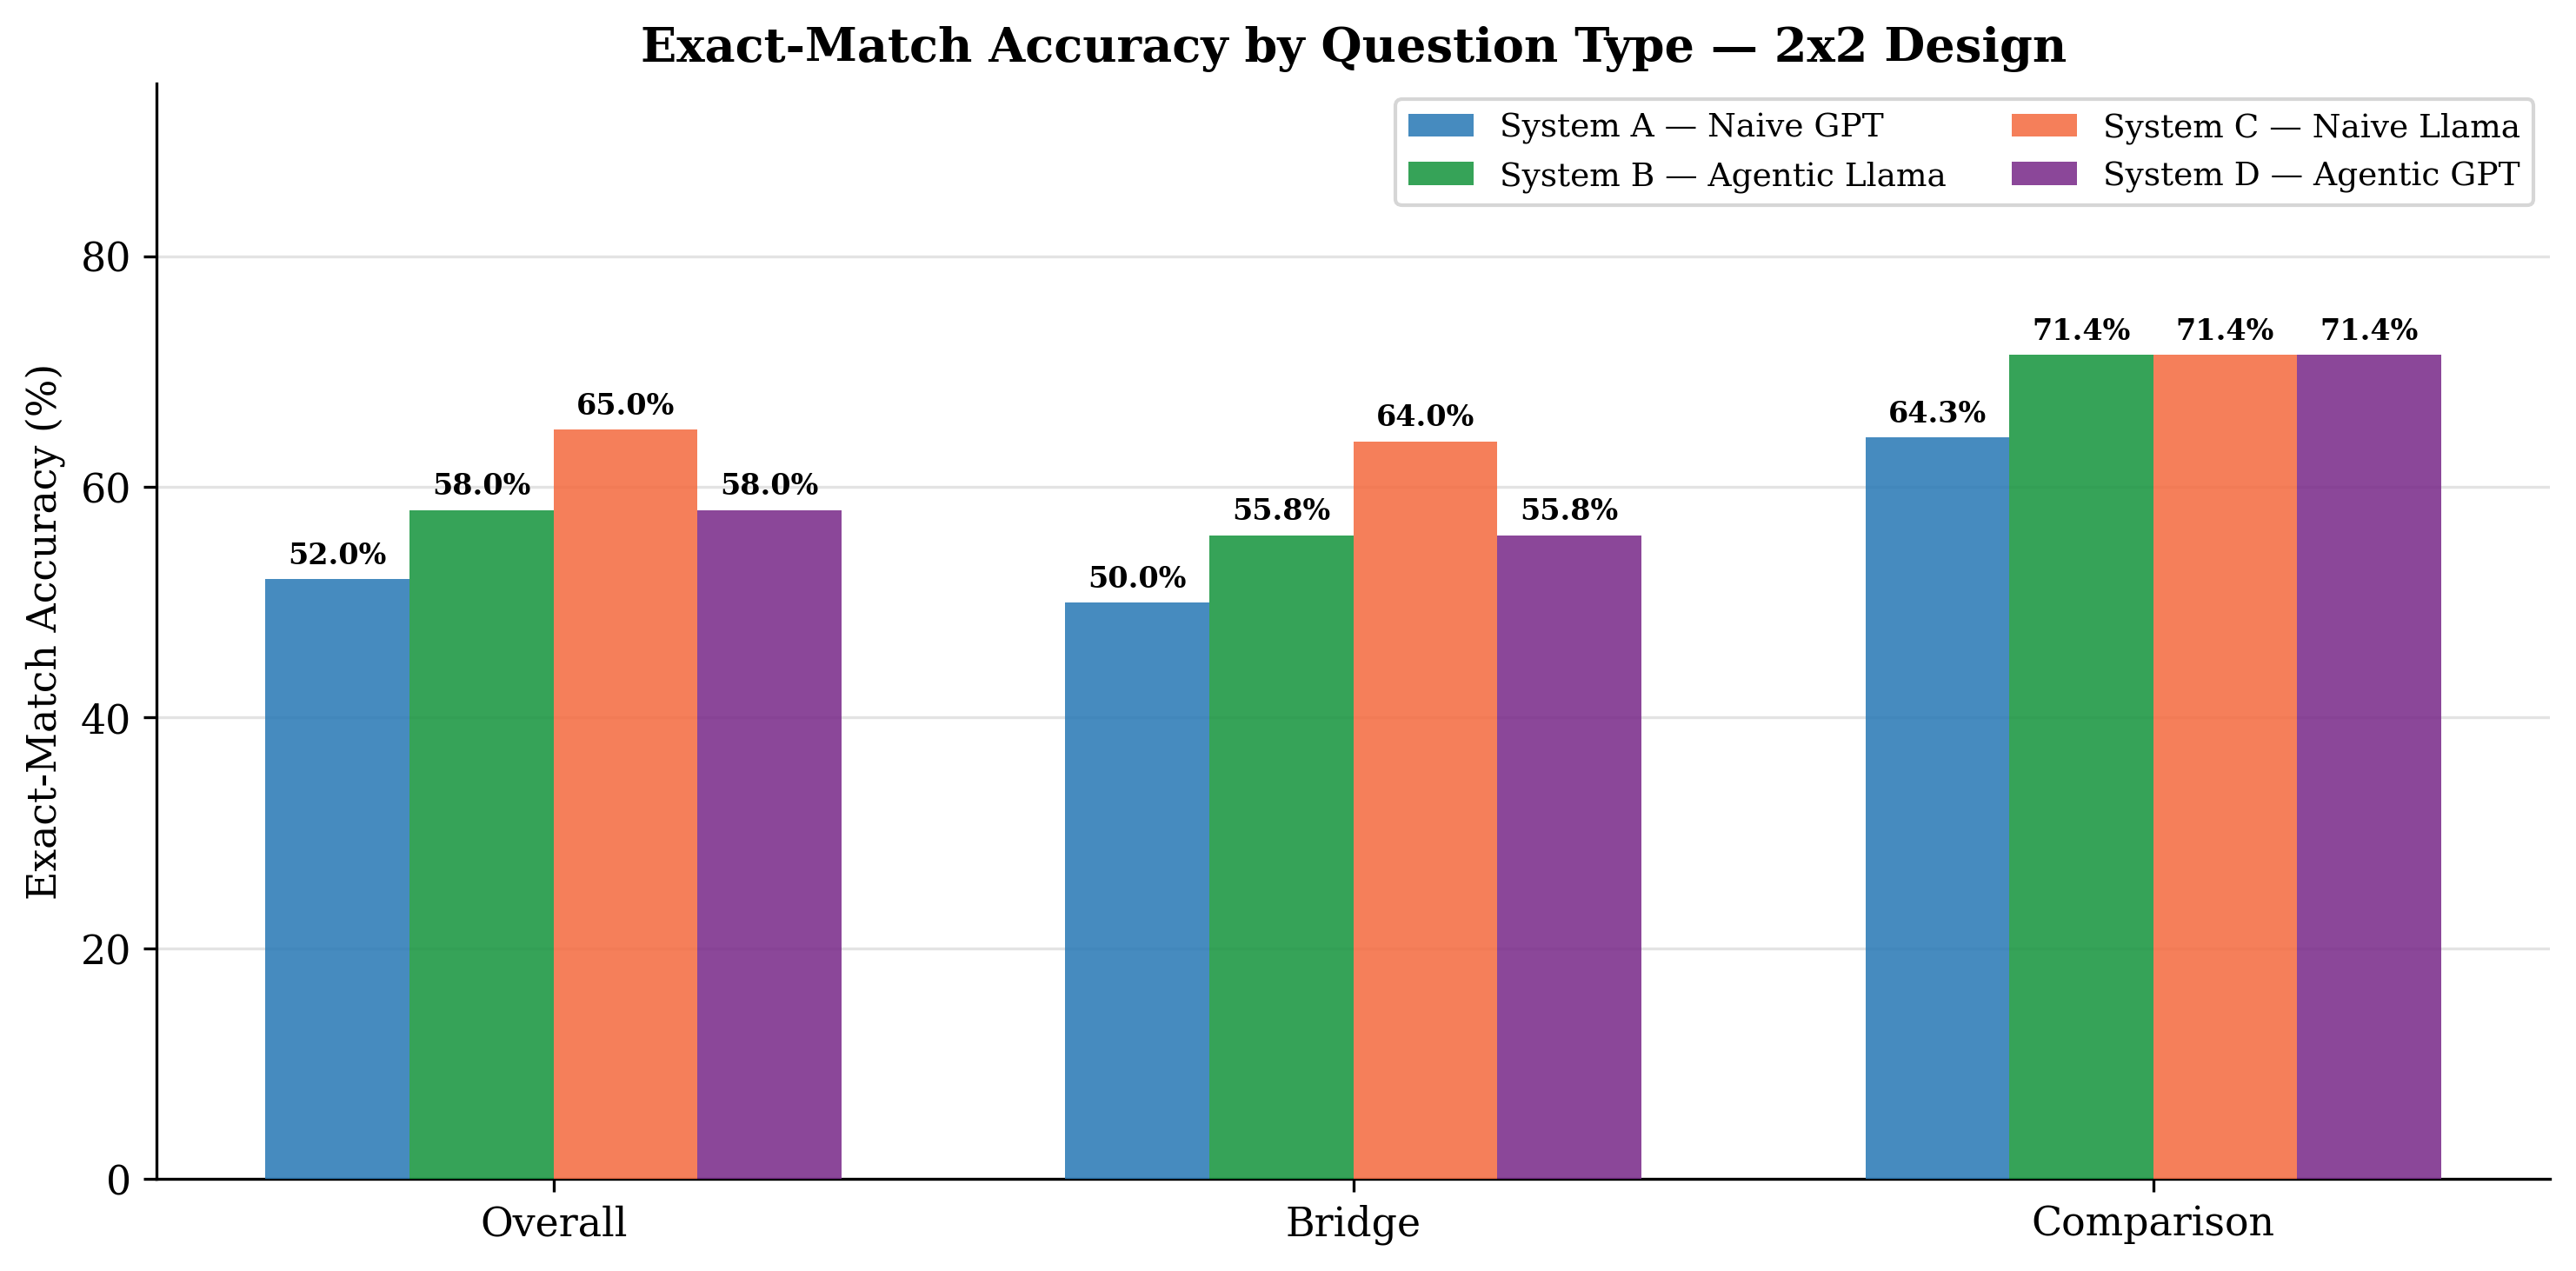
\includegraphics[width=0.92\textwidth]{../evaluation/results/chart_exact_match.png}
\caption{Exact-match accuracy by question type for all four systems.  System C
(Hermes --- Naive Llama) achieves the highest overall accuracy (65.0\%) across
both bridge and comparison questions.}
\label{fig:exactmatch}
\end{figure}

\subsection{RAGAS Evaluation}

\begin{table}[H]
\centering
\caption{RAGAS Metric Scores --- All Four Systems}
\label{tab:ragas}
\rowcolors{2}{lightgray}{white}
\begin{tabular}{lcccc}
\toprule
\textbf{Metric} & \textbf{A (Goliath)} & \textbf{B (David)} &
\textbf{C (Hermes)} & \textbf{D (Titan)} \\
\midrule
Faithfulness
  & 0.6025
  & 0.7135
  & \textcolor{wingreen}{\textbf{0.7333}}
  & 0.6431 \\
Answer Relevancy
  & 0.6595
  & 0.5159
  & 0.5405
  & \textcolor{wingreen}{\textbf{0.6882}} \\
Context Precision
  & 0.6642
  & 0.6882
  & 0.6523
  & \textcolor{wingreen}{\textbf{0.6896}} \\
Context Recall
  & 0.7500
  & 0.7400
  & 0.7600
  & \textcolor{wingreen}{\textbf{0.7700}} \\
\midrule
\textbf{Metrics Won}\textsuperscript{$\dagger$}
  & 0/4
  & 0/4
  & 1/4
  & \textcolor{wingreen}{\textbf{3/4}} \\
\bottomrule
\multicolumn{5}{l}{\footnotesize $\dagger$ Magnitudes of leads vary; this row indicates direction only.}
\end{tabular}
\end{table}

\begin{figure}[H]
\centering
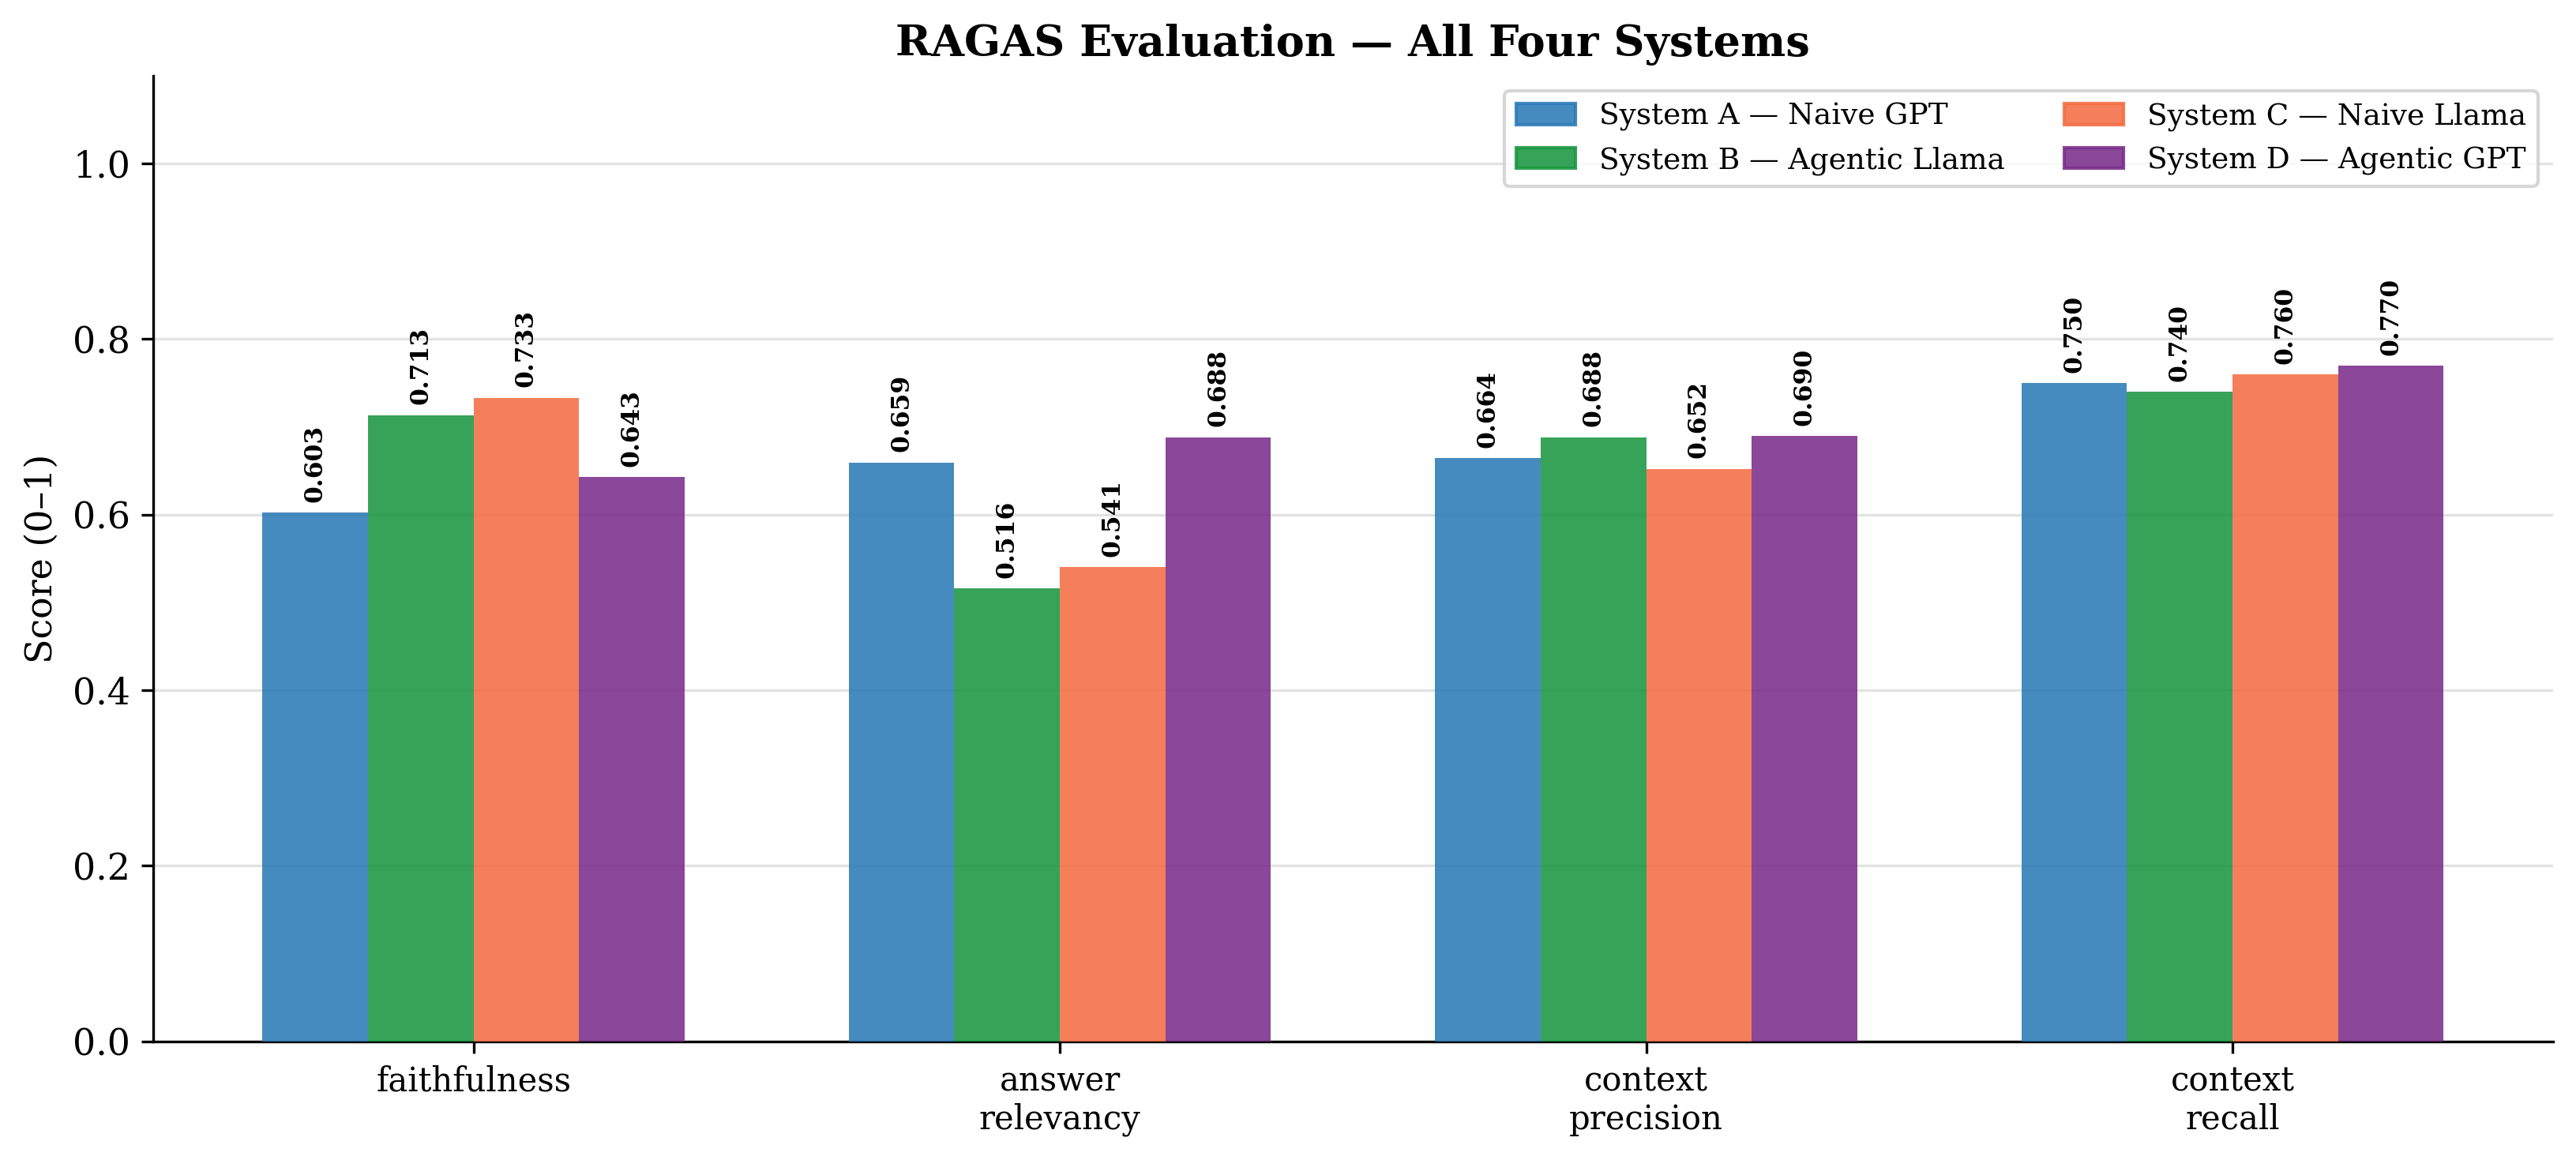
\includegraphics[width=\textwidth]{../evaluation/results/chart_ragas.png}
\caption{RAGAS metric comparison across all four systems.  System C (Hermes)
leads on faithfulness; System D (Titan) leads on answer relevancy, context
precision, and context recall.}
\label{fig:ragas}
\end{figure}

\subsection{The 2$\times$2 Interaction Effect}

The central finding of this study is that scale and architecture do not combine
additively---they \emph{interact}.

\begin{figure}[H]
\centering
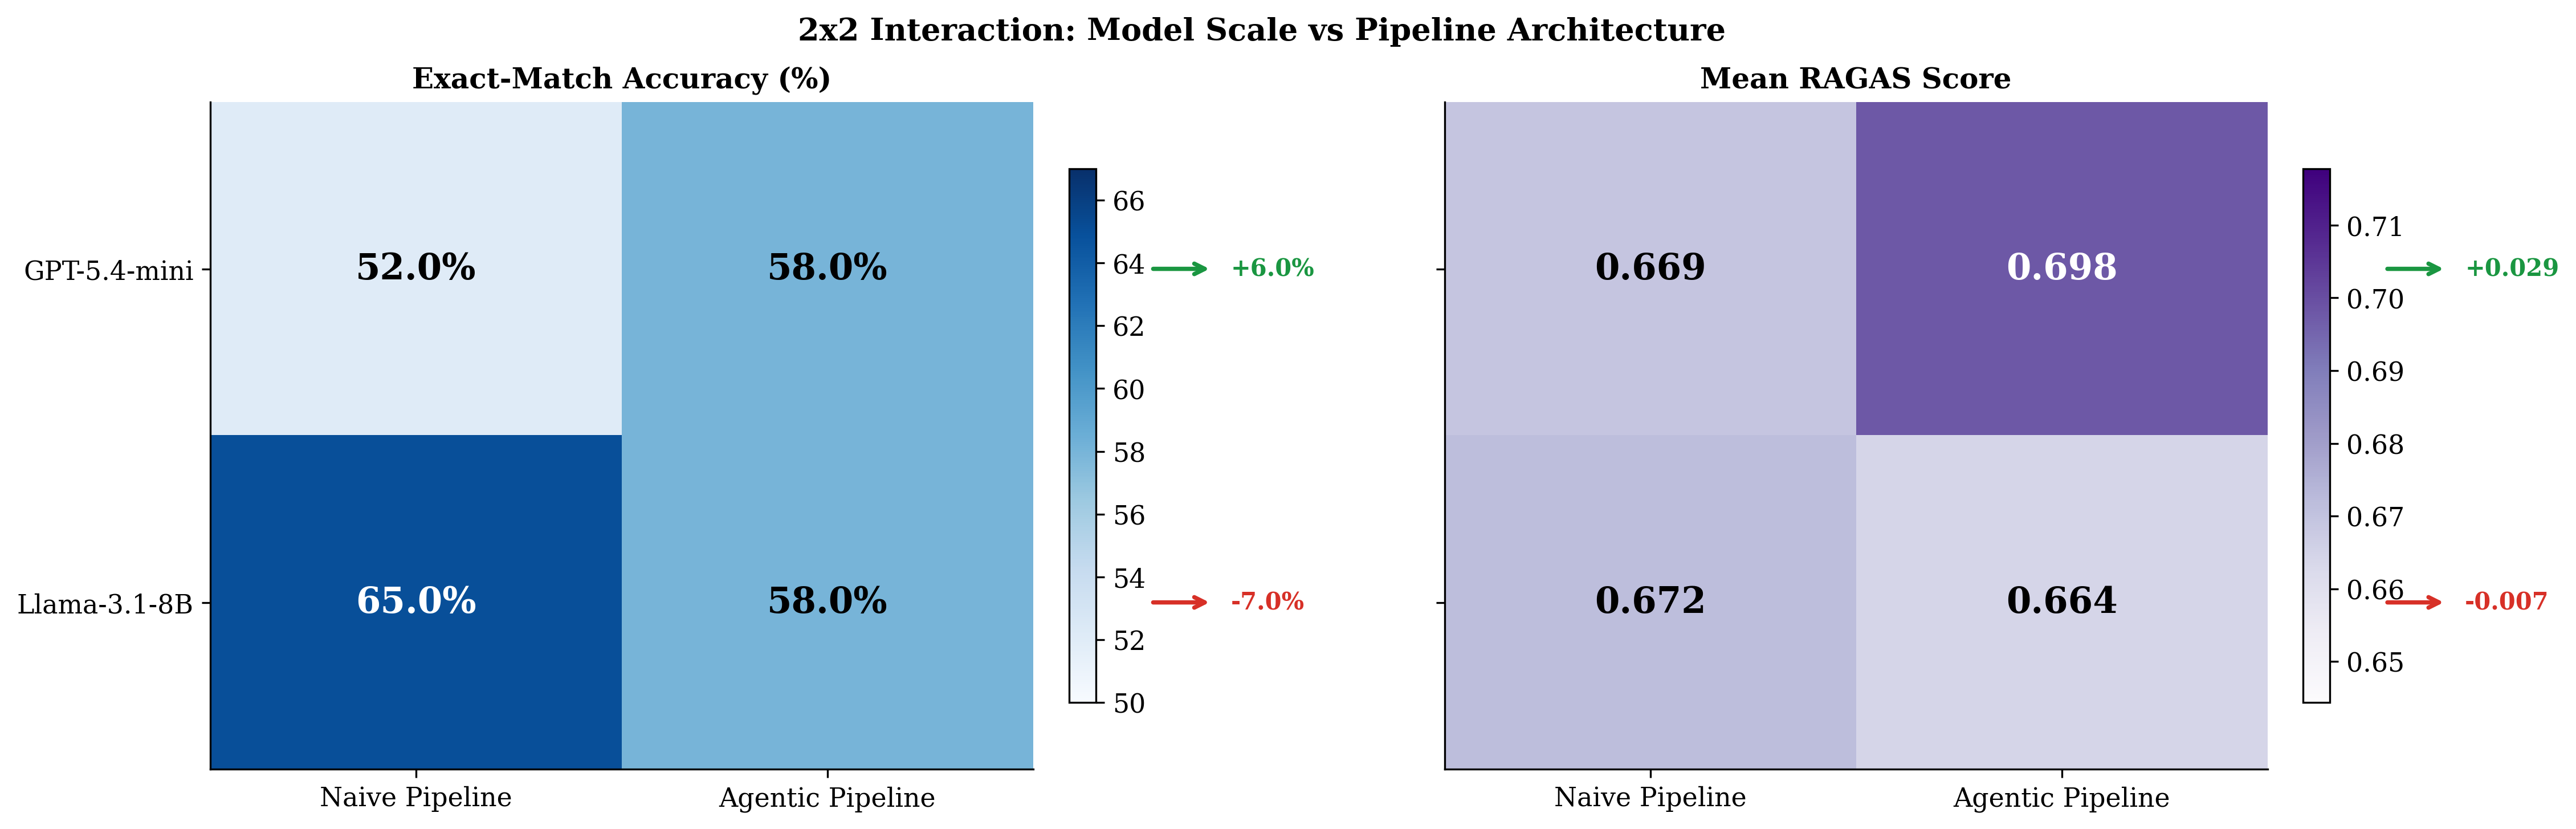
\includegraphics[width=\textwidth]{../evaluation/results/chart_2x2_interaction.png}
\caption{2$\times$2 interaction heatmaps.  \textit{Left}: exact-match accuracy.
\textit{Right}: mean RAGAS score.  Arrows show the effect of switching from
naive to agentic pipeline within each model family.  The agentic pipeline
\emph{helps} GPT but \emph{hurts} Llama on EM; results are more nuanced on
RAGAS.}
\label{fig:interaction}
\end{figure}

Table~\ref{tab:interaction} quantifies the main effects and interaction:

\begin{table}[H]
\centering
\caption{Main Effects and Interaction (Exact-Match Accuracy)}
\label{tab:interaction}
\begin{tabular}{lcc}
\toprule
\textbf{Effect} & \textbf{Naive} & \textbf{Agentic} \\
\midrule
GPT-5.4-mini row & 52.0\% (A) & 58.0\% (D) \quad $\Delta = +6.0$pp \\
Llama-3.1-8B row & \textbf{65.0\%} (C) & 58.0\% (B) \quad $\Delta = -7.0$pp \\
\midrule
\multicolumn{3}{l}{\textbf{Interaction}: $+6.0 - (-7.0) = 13.0$pp
  \quad (agentic benefits GPT more than Llama)} \\
\bottomrule
\end{tabular}
\end{table}

The 13-percentage-point interaction term is the key result: the agentic
pipeline is far from model-agnostic.

\subsection{Summary of Results}

\begin{table}[H]
\centering
\caption{Full Metric Summary}
\label{tab:summary}
\begin{tabular}{lcccc}
\toprule
\textbf{Metric} & \textbf{A (Goliath)} & \textbf{B (David)} &
\textbf{C (Hermes)} & \textbf{D (Titan)} \\
\midrule
EM Overall          & 52.0\% & 58.0\% & \textcolor{wingreen}{\textbf{65.0\%}} & 58.0\% \\
EM Bridge           & 50.0\% & 55.8\% & \textcolor{wingreen}{\textbf{64.0\%}} & 55.8\% \\
EM Comparison       & 64.3\% & 71.4\% & \textcolor{wingreen}{\textbf{71.4\%}} & \textcolor{wingreen}{\textbf{71.4\%}} \\
RAGAS Faithfulness  & 0.603  & 0.714  & \textcolor{wingreen}{\textbf{0.733}} & 0.643 \\
RAGAS Ans.\ Rel.    & 0.660  & 0.516  & 0.541 & \textcolor{wingreen}{\textbf{0.688}} \\
RAGAS Ctx.\ Prec.   & 0.664  & 0.688  & 0.652 & \textcolor{wingreen}{\textbf{0.690}} \\
RAGAS Ctx.\ Rec.    & 0.750  & 0.740  & 0.760 & \textcolor{wingreen}{\textbf{0.770}} \\
Completion Rate     & \textcolor{wingreen}{\textbf{100\%}} &
                      \textcolor{wingreen}{\textbf{100\%}} &
                      \textcolor{wingreen}{\textbf{100\%}} &
                      \textcolor{wingreen}{\textbf{100\%}} \\
\bottomrule
\end{tabular}
\end{table}

\subsection{Agentic Loop Behaviour}
\label{sec:loop}

\begin{table}[H]
\centering
\caption{Agentic Loop Statistics ($n = 100$ questions each)}
\label{tab:loop}
\rowcolors{2}{lightgray}{white}
\begin{tabular}{lcc}
\toprule
\textbf{Statistic} & \textbf{System B (David)} & \textbf{System D (Titan)} \\
\midrule
Mean retrieval attempts   & 2.78 & 2.76 \\
Mean generation attempts  & 1.07 & 1.31 \\
\bottomrule
\end{tabular}
\end{table}

\begin{figure}[H]
\centering
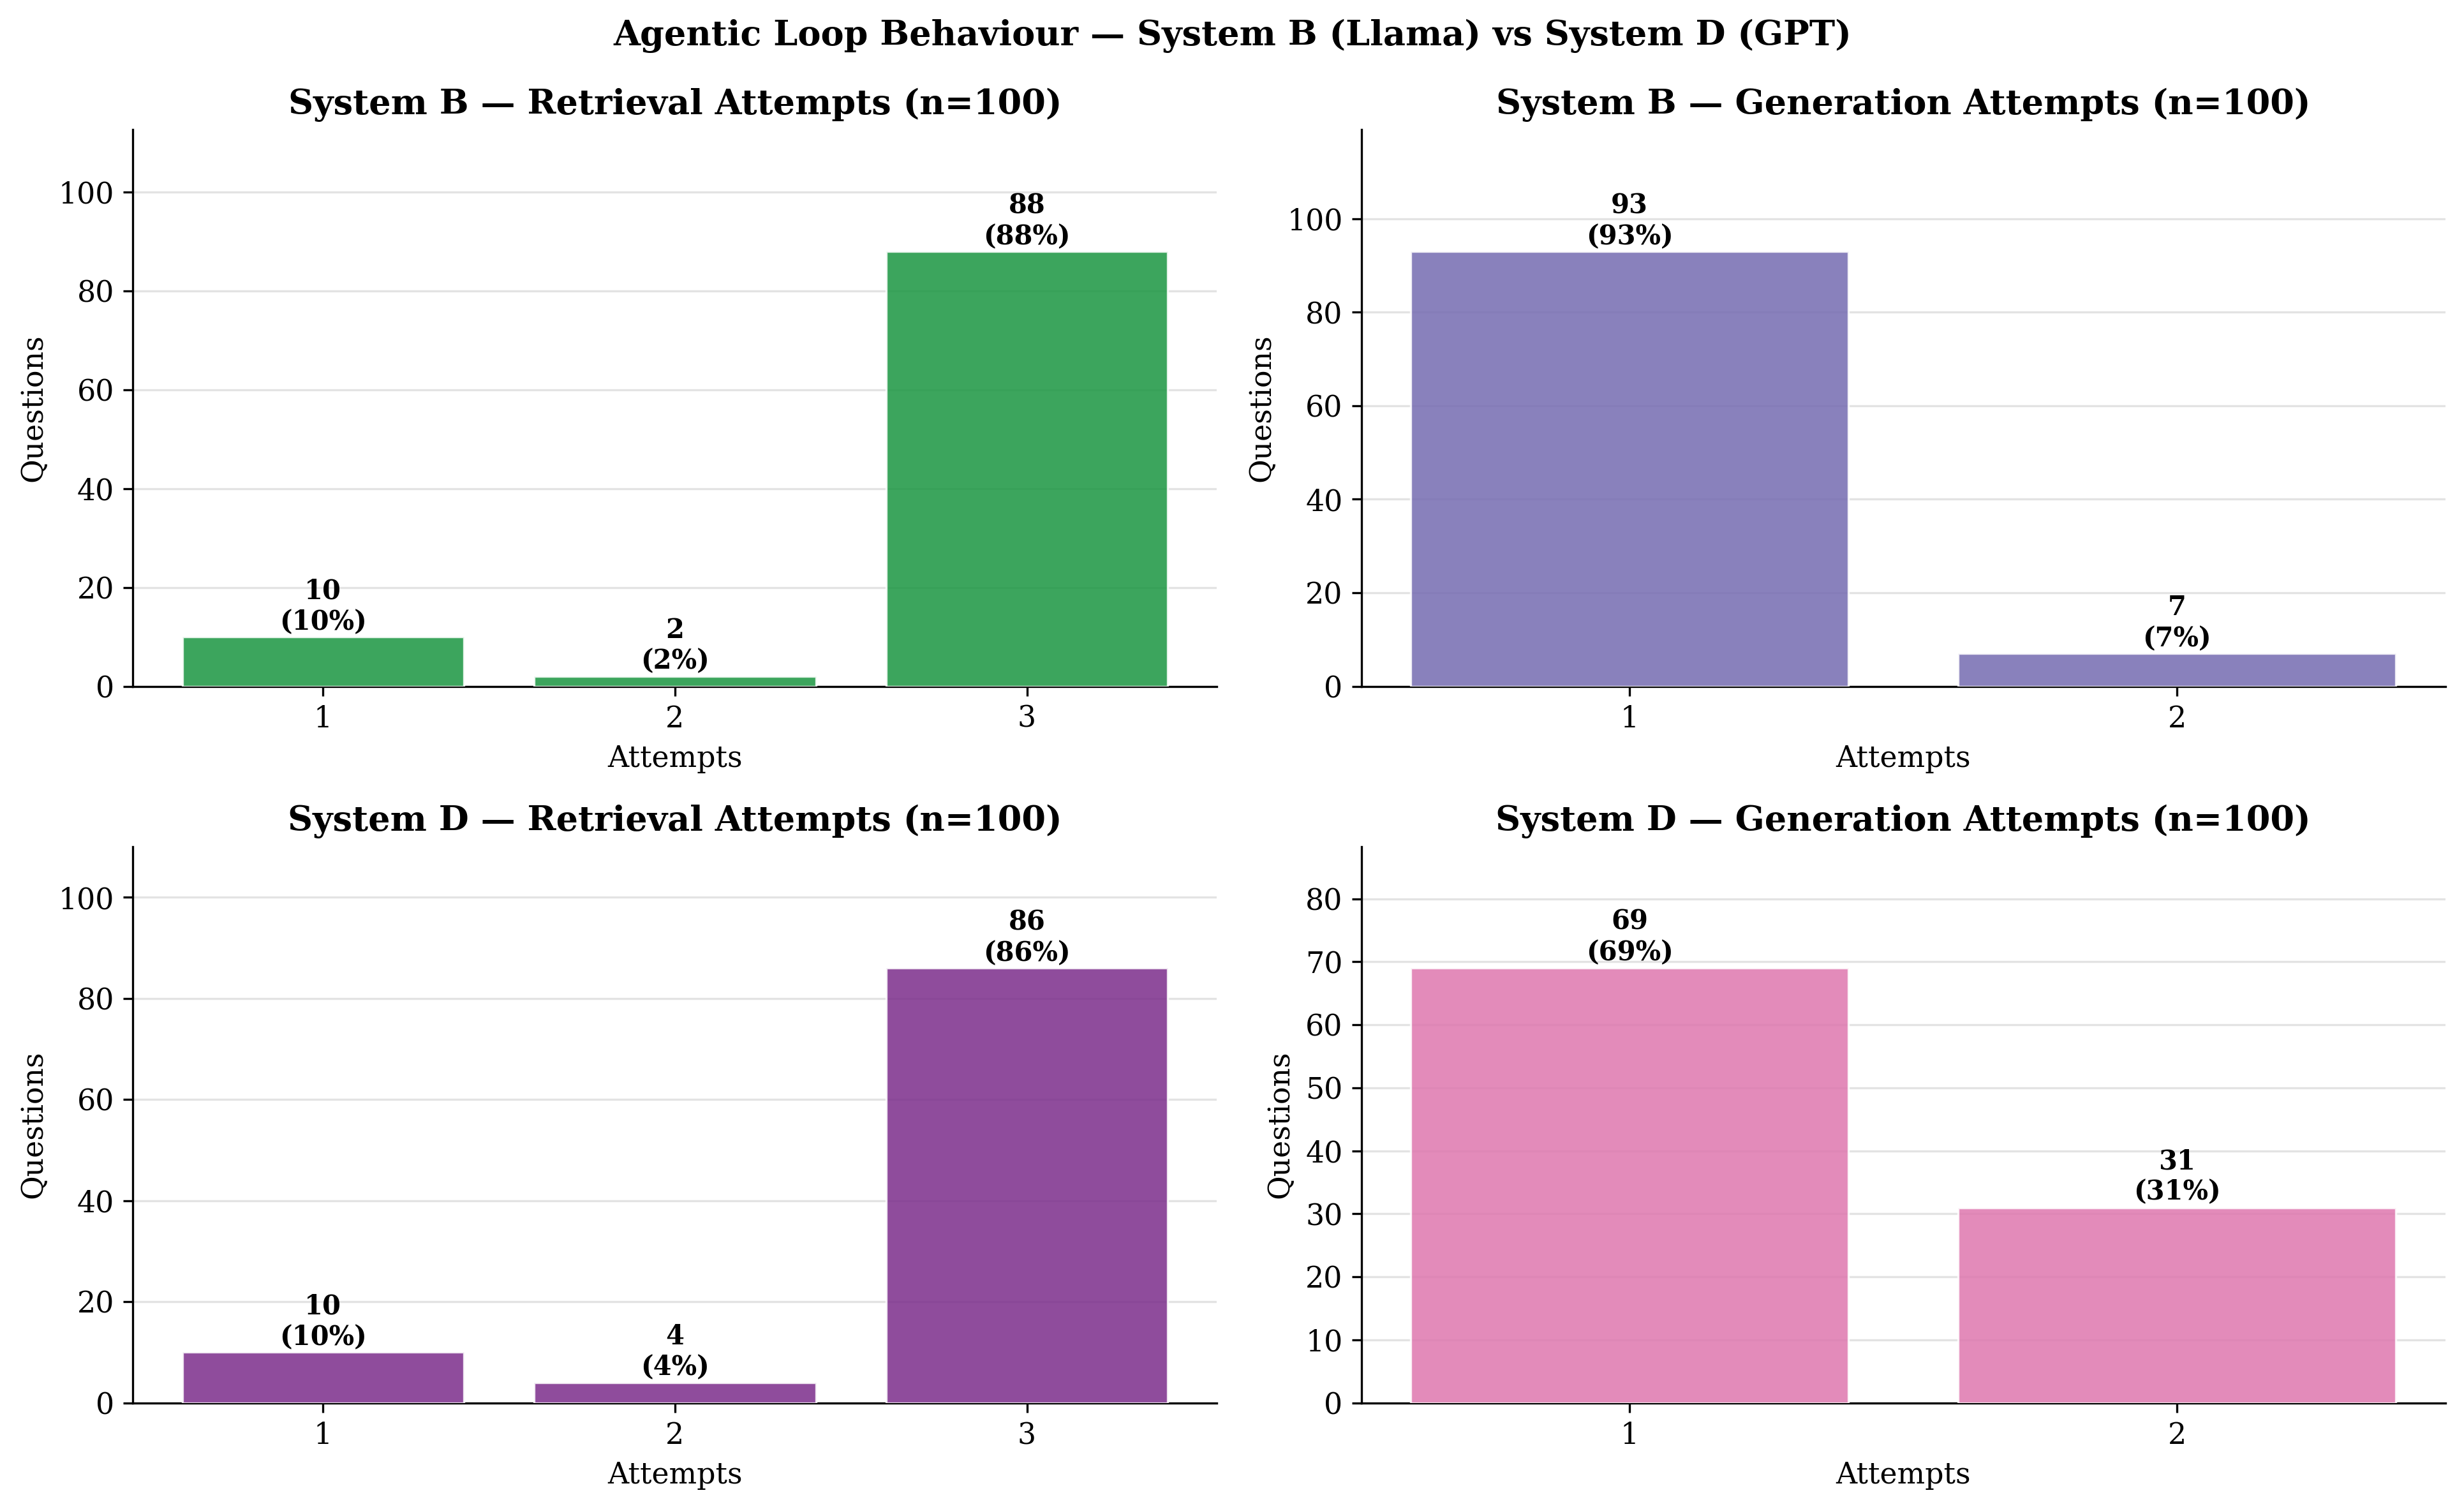
\includegraphics[width=\textwidth]{../evaluation/results/chart_loop_behaviour.png}
\caption{Agentic loop behaviour for System B (Llama) and System D (GPT) across
100 questions.  Both systems exhaust the retrieval ceiling at similar rates.
System D triggers significantly more regeneration passes (mean 1.31 vs 1.07),
reflecting GPT's stricter hallucination detection.}
\label{fig:loop}
\end{figure}

Both agentic systems exhaust the retrieval budget at similar rates
(2.78 vs 2.76 mean attempts), indicating that the retrieval bottleneck is
driven by the distractor corpus structure rather than model capability.  However,
System D (GPT) triggers substantially more regeneration passes than System B
(Llama): mean 1.31 vs 1.07.  This suggests that GPT's hallucination checker
is stricter and more accurate---it correctly identifies unsupported claims and
demands regeneration, whereas Llama's checker is more permissive and often
accepts a flawed first draft.

%──────────────────────────────────────────────────────────────────────────────
\section{Discussion}
%──────────────────────────────────────────────────────────────────────────────

\subsection{Evidence for a Capability Threshold in Self-Correction}

The most important finding of this paper is the model-by-pipeline interaction.
The agentic pipeline imposes several complex reasoning demands beyond simple
generation: it requires the model to \emph{grade} retrieved passages
for relevance, \emph{rewrite} queries when retrieval fails, and
\emph{verify} factual grounding in its own output.  These tasks require
meta-cognitive ability that may exceed the capacity of smaller models.

Llama-3.1-8B appears to fall below a \textbf{capability threshold} for
productive self-correction.  Evidence for this comes from three observations:
(1) the agentic pipeline \emph{hurts} Llama on EM ($-7.0$pp), while it helps
GPT ($+6.0$pp); (2) Llama's hallucination checker is permissive, accepting
first drafts at a high rate (mean 1.07 generation attempts vs 1.31 for GPT),
suggesting it does not reliably detect unsupported claims; and (3) Naive Llama
(65.0\% EM) outperforms Agentic Llama (58.0\% EM), meaning the self-correction
loop introduces more errors than it corrects.

\subsection{Why Naive Llama Wins on Exact-Match}

The result that Hermes (Naive Llama, 65.0\% EM) outperforms all GPT variants
on exact-match accuracy is counterintuitive.  We attribute this to two factors.
First, Llama-3.1-8B's responses tend to be more concise and direct, making
exact-match---a substring check---more likely to succeed.  GPT-5.4-mini often
produces fluent but verbose answers that restate the question or add context,
causing the short ground-truth string to be absent even when the answer is
semantically correct.  Second, the distractor corpus structure may favour
Llama's pattern-matching behaviour on HotpotQA's factoid question style.

This finding highlights a known limitation of exact-match as an evaluation
metric: it penalises verbosity even when the underlying answer is correct.
The RAGAS metrics, which evaluate semantic quality rather than string overlap,
tell a different story: System D (Agentic GPT) leads on three of four RAGAS
metrics, suggesting it produces higher-quality answers that happen to be
phrased differently from the ground truth.

\subsection{Faithfulness vs.\ Answer Relevancy Trade-off}

An interesting split emerges on RAGAS metrics: Hermes (Naive Llama) leads on
\emph{faithfulness} (0.733), while Titan (Agentic GPT) leads on
\emph{answer relevancy} (0.688).  Faithfulness measures whether every claim
in the answer is grounded in retrieved context; answer relevancy measures
whether the answer actually addresses the question.  Llama's higher faithfulness
may reflect a tendency to stay closely anchored to the retrieved text (avoiding
hallucination by paraphrasing directly), while GPT's higher answer relevancy
reflects its stronger instruction-following and question-interpretation ability.
The agentic pipeline's hallucination checker further reinforces faithfulness in
both systems.

\subsection{Implications for Practitioners}

\begin{itemize}
    \item \textbf{Match pipeline complexity to model capability.}  An agentic
          self-correction loop is not universally beneficial.  It requires the
          model to perform document grading, query rewriting, and hallucination
          verification reliably.  For smaller models such as Llama-3.1-8B, a
          well-tuned naive pipeline may outperform an agentic one.
    \item \textbf{Evaluate metrics carefully.}  Exact-match favours concise
          models; RAGAS metrics favour semantically accurate but potentially
          verbose ones.  Use multiple complementary metrics before concluding
          which system is ``better.''
    \item \textbf{Local GPU inference eliminates rate limits.}  Running Llama
          on a Tesla T4 via Ollama achieved 100\% completion at effectively
          zero marginal cost, compared to the 30.5\% failure rate observed
          with cloud API inference.  This is a practical recommendation for
          any project that issues high volumes of LLM calls.
    \item \textbf{Naive RAG remains competitive.}  Despite the attention
          agentic systems receive, a simple retrieve-then-generate pipeline
          with a capable model or a concise smaller model remains a strong
          baseline that should not be dismissed.
\end{itemize}

\subsection{Limitations}

\begin{itemize}
    \item \textbf{Single benchmark.}  Results are specific to HotpotQA
          multi-hop distractor QA.  The interaction effect may differ on
          single-hop, conversational, or domain-specific benchmarks.
    \item \textbf{Exact-match conservatism.}  The substring EM metric
          under-credits verbose but correct answers, systematically
          disadvantaging GPT systems.
    \item \textbf{Single experimental run.}  No confidence intervals are
          reported.  Despite temperature 0, minor variance may exist across runs.
    \item \textbf{Quantised local model.}  The Llama model served via Ollama
          uses 4-bit quantisation, which may introduce small accuracy penalties
          relative to the full-precision model used via cloud APIs.
    \item \textbf{Single model pair.}  The capability threshold hypothesis
          requires further validation with additional model sizes
          (e.g., Llama-3.1-70B, Llama-3.2-3B) to establish where the
          threshold lies.
    \item \textbf{Small comparison-question subset.}  Only 14 of the 100
          sampled questions are of the comparison type; results broken down
          by question type for this subset should be read as indicative
          rather than definitive.
\end{itemize}

%──────────────────────────────────────────────────────────────────────────────
\section{Future Work}
%──────────────────────────────────────────────────────────────────────────────

\begin{itemize}
    \item \textbf{Capability threshold study.}  Systematically varying model
          size (1B, 3B, 8B, 13B, 70B parameters) within the same agentic
          pipeline to identify the parameter count at which self-correction
          becomes productive.
    \item \textbf{Full-scale evaluation.}  Running on the full HotpotQA
          validation set (7{,}405 questions) for statistically robust results.
    \item \textbf{Comparison with other agentic frameworks.}  Contrasting
          LangGraph self-correction with ReAct~\cite{yao2022react},
          Self-RAG~\cite{asai2023selfrag}, and Reflexion~\cite{shinn2023reflexion}.
    \item \textbf{Semantic evaluation.}  Replacing or supplementing exact-match
          with model-based semantic equivalence scoring to reduce the verbosity
          penalty on GPT systems.
    \item \textbf{Cost-performance analysis.}  Measuring API cost and inference
          latency per correct answer across all four systems to compute a
          cost-adjusted performance frontier.
\end{itemize}

%──────────────────────────────────────────────────────────────────────────────
\section{Conclusion}
%──────────────────────────────────────────────────────────────────────────────

This paper presented a controlled 2$\times$2 factorial study crossing two
model families (GPT-5.4-mini, Llama-3.1-8B) with two pipeline architectures
(naive RAG, agentic self-correcting RAG) on the HotpotQA distractor benchmark.

The central finding is a \textbf{13-percentage-point interaction effect} in
exact-match accuracy: agentic self-correction improves GPT-5.4-mini by 6
percentage points but degrades Llama-3.1-8B by 7 percentage points.  This
result challenges the assumption that agentic pipelines are universally
beneficial, suggesting instead that iterative self-correction requires a
\emph{capability threshold} in the underlying model that Llama-3.1-8B does
not reliably meet.  Practically, Hermes (Naive Llama) achieves the highest
overall exact-match accuracy (65.0\%), demonstrating that a simpler pipeline
with a well-matched model can outperform more complex alternatives.

On RAGAS metrics, the picture is more nuanced: Titan (Agentic GPT) leads on
answer relevancy, context precision, and context recall, while Hermes leads
on faithfulness---suggesting a faithfulness-vs-relevancy trade-off between
the two model families.

Finally, by switching from cloud API inference to local GPU inference via
Ollama on a Tesla T4, we achieved 100\% completion across all four systems,
eliminating the rate-limit failures that have confounded earlier comparisons
of agentic RAG systems.

Our results suggest that practitioners and researchers should choose an agentic
pipeline based on their model's self-correction capability, rather than assuming
that more complexity is always better.

%──────────────────────────────────────────────────────────────────────────────
\begin{thebibliography}{00}
%──────────────────────────────────────────────────────────────────────────────

\bibitem{lewis2020retrieval}
P.\ Lewis et al., ``Retrieval-augmented generation for knowledge-intensive NLP
tasks,'' \textit{Advances in Neural Information Processing Systems}, vol.~33,
pp.~9459--9474, 2020.

\bibitem{karpukhin2020dense}
V.\ Karpukhin et al., ``Dense passage retrieval for open-domain question
answering,'' in \textit{Proc.\ EMNLP}, 2020, pp.~6769--6781.

\bibitem{yang2018hotpotqa}
Z.\ Yang et al., ``HotpotQA: A dataset for diverse, explainable multi-hop
question answering,'' in \textit{Proc.\ EMNLP}, 2018, pp.~2369--2380.

\bibitem{brown2020gpt3}
T.\ Brown et al., ``Language models are few-shot learners,''
\textit{Advances in Neural Information Processing Systems}, vol.~33,
pp.~1877--1901, 2020.

\bibitem{kaplan2020scaling}
J.\ Kaplan et al., ``Scaling laws for neural language models,''
\textit{arXiv preprint arXiv:2001.08361}, 2020.

\bibitem{yao2022react}
S.\ Yao et al., ``ReAct: Synergizing reasoning and acting in language models,''
in \textit{Proc.\ ICLR}, 2023.

\bibitem{shinn2023reflexion}
N.\ Shinn et al., ``Reflexion: Language agents with verbal reinforcement
learning,'' \textit{Advances in Neural Information Processing Systems},
vol.~36, 2023.

\bibitem{asai2023selfrag}
A.\ Asai et al., ``Self-RAG: Learning to retrieve, generate, and critique
through self-reflection,'' in \textit{Proc.\ ICLR}, 2024.

\bibitem{es2023ragas}
S.\ Es et al., ``RAGAS: Automated evaluation of retrieval augmented
generation,'' \textit{arXiv preprint arXiv:2309.15217}, 2023.

\end{thebibliography}

\end{document}
